%!TEX program = pdflatex
\documentclass[12pt]{extarticle}
\usepackage[english]{babel}
\usepackage{graphicx}
\usepackage{framed}
\usepackage[normalem]{ulem}
\usepackage{amsmath}
\usepackage{amsthm}
\usepackage{amssymb}
\usepackage{amsfonts}
\usepackage{enumerate}
\usepackage{enumitem}
\usepackage[utf8]{inputenc}
\usepackage[top=1in,bottom=1in,left=1in,right=1in]{geometry}
\usepackage{mdframed}
\usepackage{xcolor}
\usepackage{listings}
\usepackage[numbered,framed]{matlab-prettifier}
\usepackage{hyperref}
\graphicspath{.}
\hypersetup{
  colorlinks=true,
  linkcolor=blue
}
\theoremstyle{definition}
\newtheorem{exercise}{Exercise}
\everymath{\displaystyle}

\newcommand{\ones}{\mathbf 1}
\newcommand{\E}{\mathop{\bf E{}}}          % not used now
\newcommand{\R}{\mathbb{R}}
\newcommand{\Z}{\mathbb{Z}}
\newcommand{\D}{\mathcal{D}}
\newcommand{\symm}{\mathbb{S}}
\newcommand{\<}{\langle}
\renewcommand{\>}{\rangle}

\newcommand{\nullspace}{{\mathcal N}}      % not used now
\newcommand{\range}{{\mathcal R}}          % not used now
\newcommand{\Rank}{\mathop{\bf Rank}}      % not used now
\newcommand{\tr}{\mathop{\bf tr}}
\newcommand{\diag}{\mathop{\bf diag}}
\newcommand{\card}{\mathop{\bf card}}      % not used now
\newcommand{\rank}{\mathop{\bf rank}}      % not used now
\newcommand{\aff}{\mathop{\bf aff}}
\newcommand{\conv}{\mathop{\bf conv}}
\newcommand{\prox}{\mathbf{prox}}
\newcommand{\prob}{\mathop{\bf prob}}      % not used now
\newcommand{\dist}{\mathop{\bf dist{}}}
\newcommand{\argmin}{\mathop{\rm argmin}}  % not used now
\newcommand{\argmax}{\mathop{\rm argmax}}  % not used now
\newcommand{\epi}{\mathop{\bf epi}}
\newcommand{\Vol}{\mathop{\bf vol}}        % not used now
\newcommand{\dom}{\mathop{\bf dom}}
\newcommand{\intr}{\mathop{\bf int}}
\newcommand{\bd}{\mathop{\bf bd}}
\newcommand{\relintr}{\mathop{\bf relint}}
\newcommand{\cl}{\mathop{\bf cl}}
\newcommand{\sign}{\mathop{\bf sign}}

\newcommand{\cf}{\textit{cf.}}
\newcommand{\eg}{\textit{e.g.}, }
\newcommand{\ie}{\textit{i.e.}, }
\newcommand{\etal}{\textit{et al}. }
\newcommand{\etc}{\textit{etc.}}


\title{Assignment \#7}
\author{Shao Hua, Huang 0750727\\
ECM5901 - Optimization Theory and Application}
\begin{document}
\maketitle

% Exercise 1
\textbf{Note that I use} \textsc{Matlab} \textbf{to complete the following two exercises.}
\begin{exercise}
  (Equality constrained entropy maximization.)
  Consider the equality constrained entropy maximization problem
  \begin{align*}
    \text{minimize\;\;}\quad& f(x)=\sum_{i=1}^5x_i\log x_i\\
    \text{subject to}  \quad& Ax=b
  \end{align*}
  where $A=\begin{bmatrix}4&3&2&1&0\\1&1&1&1&1\end{bmatrix}$ and $b=\begin{bmatrix}20\\15\end{bmatrix}$ with $\dom f=\R_{++}^n$.\\
  Compute the solution of the problem using the following methods.
  \begin{enumerate}[label=(\alph*)]
    \item Standard Newton method (Algorithm 10.1) with initial point $x^{(0)}=[1\;2\;3\;4\;5]^T$. (30\%)
    \item Infeasible start Newton method (Algorithm 10.2) with initial point $\nu^{(0)}=0,\;x^{(0)}=[1\;2\;3\;4\;5]^T$, and also $x^{(0)}=[5\;2\;3\;4\;5]^T$. (30\%)
  \end{enumerate}
  Verify that the two methods compute the same optimal point.
  Note that $\dom f$ is not $\R^5$ and thus in the update step of $x$, you have to check that $x+t\Delta x\in\dom f$.
\end{exercise}
\begin{proof}[Solution]
  \let\qed\relax
  Shared parameters
\begin{lstlisting}[style=Matlab-editor]
% file: hw7_1.m
A = [4 3 2 1 0; 1 1 1 1 1];
b = [20 15]';
[m, n] = size(A);
maxiters = 50;
alpha = 0.01;
beta = 0.5;
nttol = 1e-7;
\end{lstlisting}

The code and the result of (a) are shown in the next page.
\begin{lstlisting}[style=Matlab-editor]
% (a) Feasible start Newton method
x = [1 2 3 4 5]';
disp('(a) Feasible start Newton method');
disp('    Iterate optimal points and values:');
disp(['           x(0) = [ ', sprintf('%f ', x), ']']);
disp(['      optval(0) = ', num2str(sum(x.*log(x)), '%f')]);
for i = 1:maxiters
    g = log(x) + 1;
    H = diag(1 ./ x);
    KKTleft = [H A'; A zeros(m)];
    KKTright = [-g; zeros(m, 1)];
    KKTv = KKTleft \ KKTright;
    xnt = KKTv(1:n);
    fprime = g' * xnt;
    if ((-fprime / 2) < nttol)
        break;
    end
    t = 1;
    val = sum(x .* log(x));
    while true
        newx = x + t * xnt;
        if (min(newx) >= 0)
            newval = sum((newx) .* log(newx));
            if (newval < val + alpha * t * fprime)
                break;
            end
        end
        t = beta * t;
    end
    x = x + t * xnt;
    disp(['           x(', int2str(i), ') = [ ', sprintf('%f ', x), ']']);
    disp(['      optval(', int2str(i), ') = ', num2str(sum(x.*log(x)), '%f')]);
end
\end{lstlisting}

\begin{lstlisting}[style=Matlab-editor]
(a) Feasible start Newton method
Iterate optimal points and values:
       x(0) = [ 1.000000 2.000000 3.000000 4.000000 5.000000 ]
  optval(0) = 18.274498
       x(1) = [ 1.295984 1.897411 2.667326 3.789180 5.350099 ]
  optval(1) = 18.188621
       x(2) = [ 1.319344 1.873759 2.661133 3.779082 5.366682 ]
  optval(2) = 18.188216
\end{lstlisting}

Code of (b) with changing $x$ to required initial feasible point $(1,2,3,4,5)$ and infeasible point $(5,2,3,4,5)$.
\begin{lstlisting}[style=Matlab-editor]
% (b) Infeasible start Newton method with (1, 2, 3, 4, 5)
x = [1 2 3 4 5]';
nu = zeros(m, 1);
disp('(b) Infeasible start Newton method with x = (1, 2, 3, 4, 5)');
disp('    Iterate optimal points and values:');
disp(['           x(0) = [ ', sprintf('%f ', x), ']']);
disp(['      optval(0) = ', num2str(sum(x.*log(x)), '%f')]);
for i = 1:maxiters
    g = log(x) + 1;
    H = diag(1 ./ x);
    r = [g + A' * nu; A * x - b];
    KKTleft = [H A'; A zeros(m)];
    KKTright = -r;
    KKTv = KKTleft \ KKTright;
    xnt = KKTv(1:n);
    nunt = KKTv(n+1:n+m);
    t = 1;
    while true
        newx = x + t * xnt;
        newnu = nu + t * nunt;
        if (min(newx) >= 0)
            newr = [(log(newx) + 1) + A' * (newnu); A * (newx) - b];
            if norm(newr) < (1 - alpha) * norm(r)
                break;
            end
        end
        t = beta * t;
    end
    x = x + t * xnt;
    nu = nu + t * nunt;
    disp(['           x(', int2str(i), ') = [ ', sprintf('%f ', x), ']']);
    disp(['      optval(', int2str(i), ') = ', num2str(sum(x.*log(x)), '%f')]);
    if (norm(newr) < nttol)
        break;
    end
end
\end{lstlisting}
\newpage
The result of $x^{(0)}=(1,2,3,4,5)$:
\begin{lstlisting}[style=Matlab-editor]
(b) Infeasible start Newton method with x = (1, 2, 3, 4, 5)
    Iterate optimal points and values:
           x(0) = [ 1.000000 2.000000 3.000000 4.000000 5.000000 ]
      optval(0) = 18.274498
           x(1) = [ 1.295984 1.897411 2.667326 3.789180 5.350099 ]
      optval(1) = 18.188621
           x(2) = [ 1.319344 1.873759 2.661133 3.779082 5.366682 ]
      optval(2) = 18.188216
           x(3) = [ 1.319414 1.873761 2.661015 3.779032 5.366779 ]
      optval(3) = 18.188216
\end{lstlisting}

The result of $x^{(0)}=(5,2,3,4,5)$:
\begin{lstlisting}[style=Matlab-editor]
(b) Infeasible start Newton method with x = (5, 2, 3, 4, 5)
    Iterate optimal points and values:
           x(0) = [ 5.000000 2.000000 3.000000 4.000000 5.000000 ]
      optval(0) = 26.321688
           x(1) = [ 0.571943 2.489808 3.160990 3.920824 4.856435 ]
      optval(1) = 18.621276
           x(2) = [ 1.128127 2.021496 2.793087 3.836830 5.220460 ]
      optval(2) = 18.214160
           x(3) = [ 1.312610 1.878115 2.666233 3.782747 5.360294 ]
      optval(3) = 18.188250
           x(4) = [ 1.319406 1.873767 2.661020 3.779036 5.366772 ]
      optval(4) = 18.188216
           x(5) = [ 1.319414 1.873761 2.661015 3.779032 5.366779 ]
      optval(5) = 18.188216
\end{lstlisting}
\end{proof}

\newpage
% Exercise 2
\begin{exercise}
  You were asked to prove that $x^\ast=(1,1/2,-1)$ is optimal for the following optimization problem in HW\#4:
  \begin{align*}
    \text{minimize\;\;}\quad& f_0(x)=(1/2)x^TPx+q^Tx+r\\
    \text{subject to}  \quad& -1\le x_i \le 1,\;i=1,2,3
  \end{align*}
  where
  \begin{align*}
    P= \begin{bmatrix}13&12&-2\\12&17&6\\-2&6&12\end{bmatrix},\;
    q= \begin{bmatrix}-22\\-14.5\\13\end{bmatrix},\;
    r= 1.
  \end{align*}
  Implement a barrier method for solving this QP.
  Assume that the initial point is $x^{(0)}=0$.
  Plot the duality gap versus Newton steps (such as Fig. 11.4).
  Verify that the barrier method computes the optimal point. (40\%)
\end{exercise}
\begin{proof}[Solution]
  \let\qed\relax
  With readily derivation, we transform the inequality constraints to $Ax\preceq b$ where
  \begin{align*}
    A=
    \begin{bmatrix}
      1&0&0\\0&1&0\\0&0&1\\-1&0&0\\0&-1&0\\0&0&-1
    \end{bmatrix},\quad
    b=
    \begin{bmatrix}
      1\\1\\1\\1\\1\\1
    \end{bmatrix}
  \end{align*}
  Therefore, the corresponding central path problem is
  \begin{align*}
    \text{minimize}\quad tf_0(x)+\phi(x)
  \end{align*}
  where $\phi(x)=-\sum_{i=1}^6\log(b_i-a_i^Tx)$ with $a_1^T,\dots,a_6^T$ are rows of $A$\par
  Also, we know that
  \begin{gather*}
    \nabla f_0(x)=Px+q,\quad\nabla^2f_0(x)=P\\
    \nabla\phi(x)=\sum_{i=1}^6\frac{a_i}{b_i-a_i^Tx}=A^Td\quad\nabla^2\phi(x)=\sum_{i=1}^6\frac{a_ia_i^T}{(b_i-a_i^Tx)^2}=A^T\diag(d)^2A
  \end{gather*}
  where $d\in\R^6$, $d_i=1/(b_i-a_i^Tx)$.\par
  The \textsc{Matlab} code and the result are shown below.
\begin{lstlisting}[style=Matlab-editor]
% file: hw7_2.m

P = [13 12 -2; 12 17 6; -2 6 12];
q = [-22 -14.5 13]';
r = 1;
A = [1 0 0; 0 1 0; 0 0 1; -1 0 0; 0 -1 0; 0 0 -1];
b = [1 1 1 1 1 1]';
[m, n] = size(A);
maxiters = 200;
alpha = 0.01;
beta = 0.5;
nttol = 1e-6;
tol = 1e-3;
mu = 20;
t = 1;
x = [0 0 0]';
inniters = [];
gaps = [];
for i = 1:maxiters
    d = b - A * x;
    val = t * (.5 * x' * P * x + q' * x + r) - sum(log(d));
    g = t * (P * x + q) + A' * (1 ./ d);
    H = t * P + A' * diag(1 ./ d .^ 2) * A;
    xnt = -H \ g;
    fprime = g' * xnt;
    s = 1;
    dd = -A * xnt;
    while (min(d + s * dd) <= 0)
        s = beta * s;
    end
    while (t * (.5 * (x + s * xnt)' * P * (x + s * xnt) + q' * (x + s * xnt) + r) - sum(log(d + s * dd)) >= val + alpha * s * fprime)
        s = beta * s;
    end
    x = x + s * xnt;
    if ((-fprime / 2) < nttol)
        gap = m / t;
        inniters = [inniters, i];
        gaps = [gaps gap];
        if (gap < tol)
            break;
        end
        t = mu * t;
    end
    disp(['x = [ ', sprintf('%f ', x), '], val = ', num2str(((1/2) * x' * P * x + q' * x + r), '%f')]);
end
inniters = [inniters, i];
gaps = [gaps gap];
figure(1)
iters1 = [];
gaps1 = [];
for i = 1:length(gaps)-1
    iters1 = [iters1 inniters(i)-1 inniters(i+1)-1];  
    gaps1 = [gaps1 gaps(i) gaps(i)]; 
end;
iters1 = [iters1 inniters(length(gaps))-1];
gaps1 = [gaps1 gaps(length(gaps))]; 
semilogy(iters1, gaps1);
axis([0 40 1e-6 1e2]);
xlabel('Newton iterations');  ylabel('duality gap');
\end{lstlisting}
\begin{lstlisting}[style=Matlab-editor]
>> run hw7_2.m
...
...
x = [ 0.999887 0.500048 -0.999938 ], val = -21.624762
x = [ 0.999876 0.500055 -0.999938 ], val = -21.624751
x = [ 0.999875 0.500056 -0.999938 ], val = -21.624750
\end{lstlisting}
$ $
\begin{figure}[h]
  \centering
  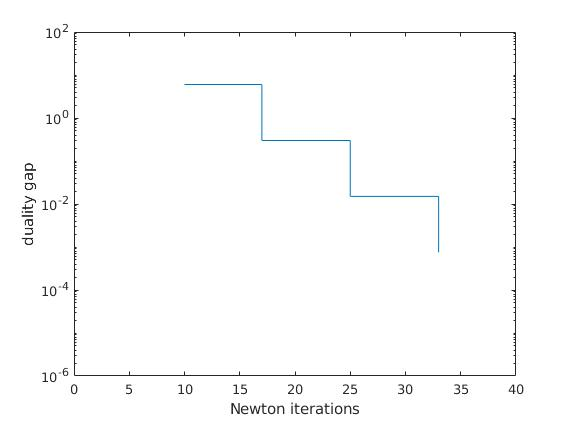
\includegraphics[width=15cm]{fig7_2}
  \caption{Relation between Newton iterations and duality gap when $\mu=20$}
\end{figure}
\end{proof}

\end{document}
